\documentclass[10pt,twocolumn,letterpaper]{article}

\usepackage{cvpr}
\usepackage{times}
\usepackage{epsfig}
\usepackage{graphicx}
\usepackage{amsmath}
\usepackage{amssymb}

% Include other packages here, before hyperref.

% If you comment hyperref and then uncomment it, you should delete
% egpaper.aux before re-running latex.  (Or just hit 'q' on the first latex
% run, let it finish, and you should be clear).
\usepackage[breaklinks=true,bookmarks=false]{hyperref}

\cvprfinalcopy % *** Uncomment this line for the final submission

\def\cvprPaperID{****} % *** Enter the CVPR Paper ID here
\def\httilde{\mbox{\tt\raisebox{-.5ex}{\symbol{126}}}}

% Pages are numbered in submission mode, and unnumbered in camera-ready
%\ifcvprfinal\pagestyle{empty}\fi
\setcounter{page}{1}
\begin{document}

%%%%%%%%% TITLE
\title{Semantic Segmentation of Urban Scenes using Fully Convolutional Networks}

\author{Zheng Luo\\
Department of Computer Science\\
University of Virginia\\
{\tt\small zl5sv@virginia.edu}
% For a paper whose authors are all at the same institution,
% omit the following lines up until the closing ``}''.
% Additional authors and addresses can be added with ``\and'',
% just like the second author.
% To save space, use either the email address or home page, not both
\and
Zixuan Lin\\
Department of Biomedical Engineering\\
University of Virginia\\
{\tt\small zl7qk@virginia.edu}
}

\maketitle
%\thispagestyle{empty}

%%%%%%%%% ABSTRACT
\begin{abstract}
   Autonomous vehicles are assumed to be the key units of the next generation transportation system. Since vehicle safety is critical to real world, it is important to maintain that a vehicle’s understanding to environment is highly reliable. Real-world driving environment is a mixture of multiple objects, and can be dense especially on urban roads. Vehicles are assumed to not only recognize multiple objects in the whole scene but also know where exactly different objects occupy. Therefore, while cameras are widely used to recognize objects, image segmentation (or clustering pixels) from a mixture becomes the challenge at the first step, in order to understand the environment precisely.
\end{abstract}




%%%%%%%%% BODY TEXT
\section{Introduction}

In this project, the plan is to cast existing different neural networks and fine tune them to segment the validation sets in Cityscapes Dataset. Finding a proper way to modify the network structures is the first important task. Moreover, we will find fine annotated training sets to train convolutional neural networks. Except playing different neural networks and compare (and try to improve) their performance of segmentation and recognition, another experiment can also be planned to test the adaptivity of trained neural networks. That is, the project is also able to study if a fine-tuned network for a single city can behave well on images from another city. Alternatively speaking, if the training set is a mixture of many different cities, it is interesting to know how much improvement can be achieved compared to only using a single or few cities.

\begin{figure}[t]
\centering
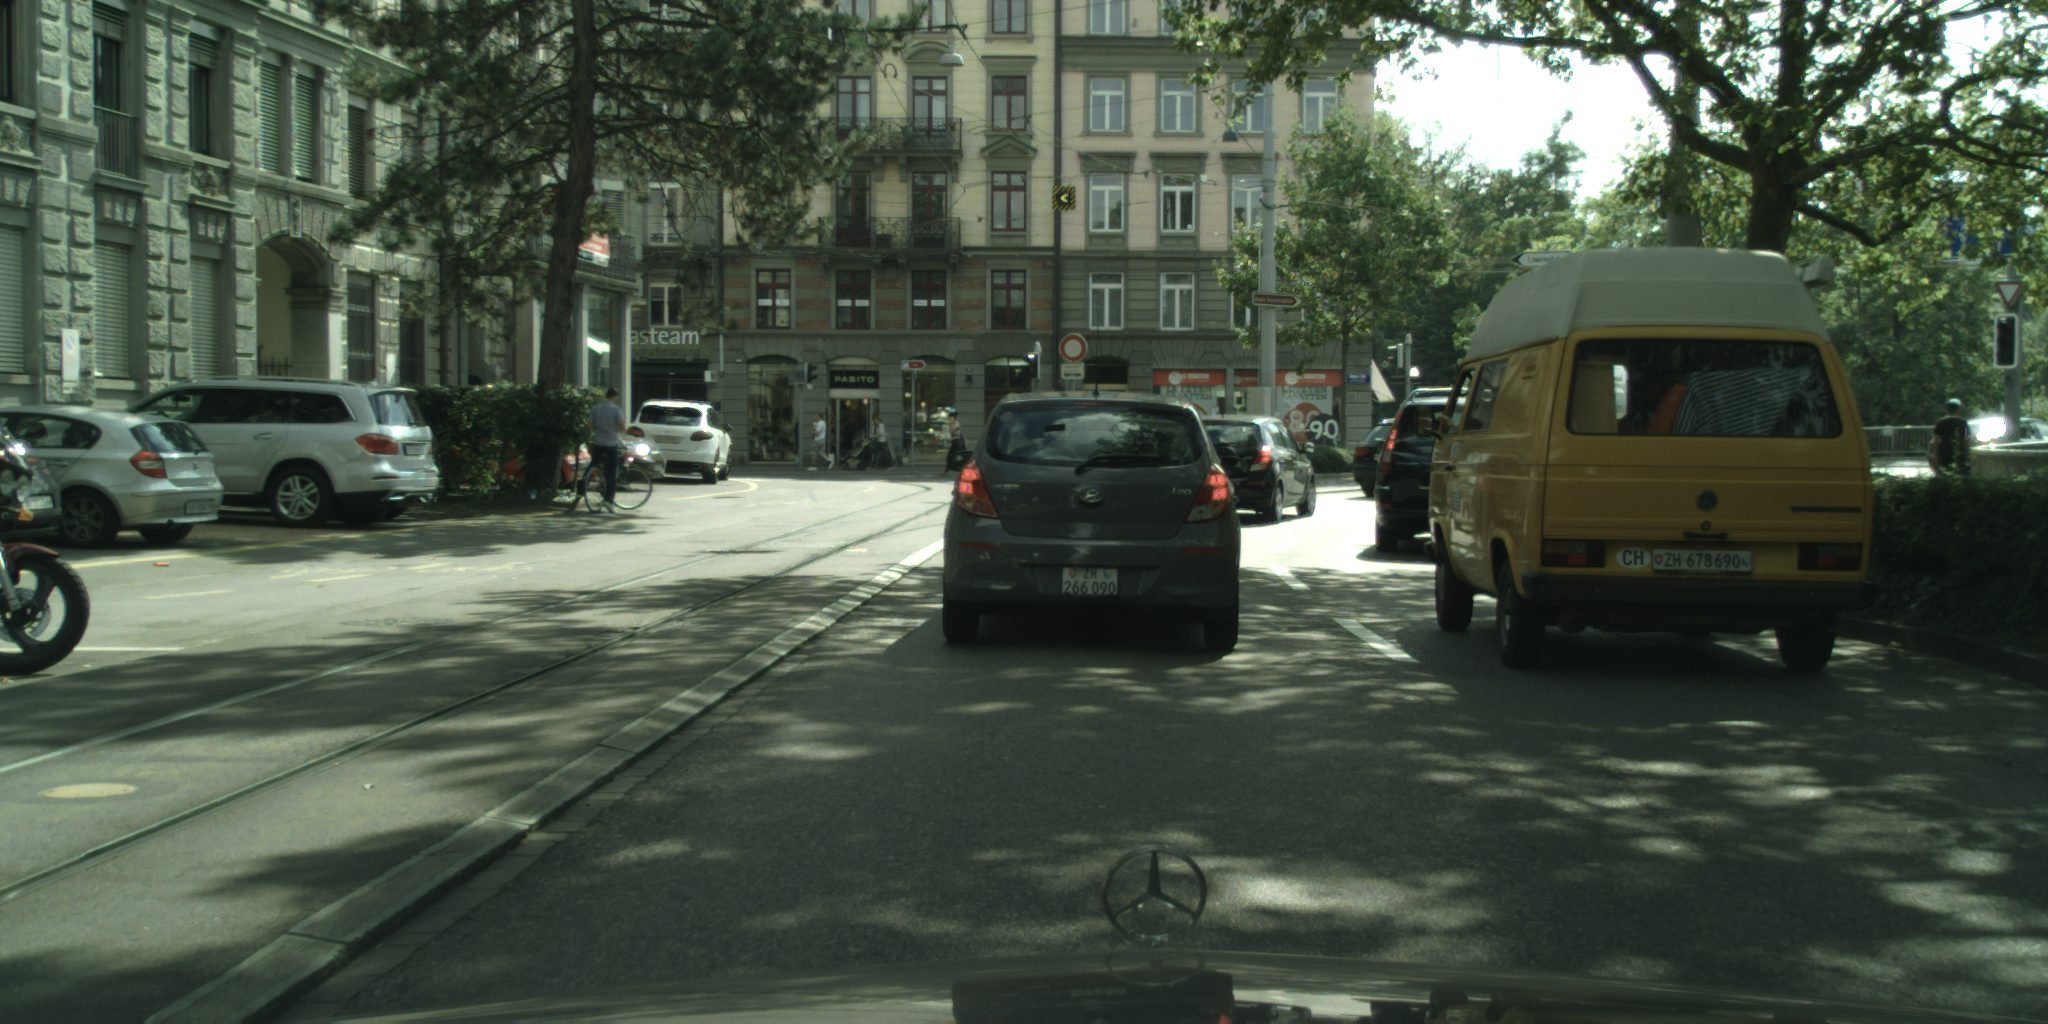
\includegraphics[width=0.40\textwidth]{zurich_example.png}
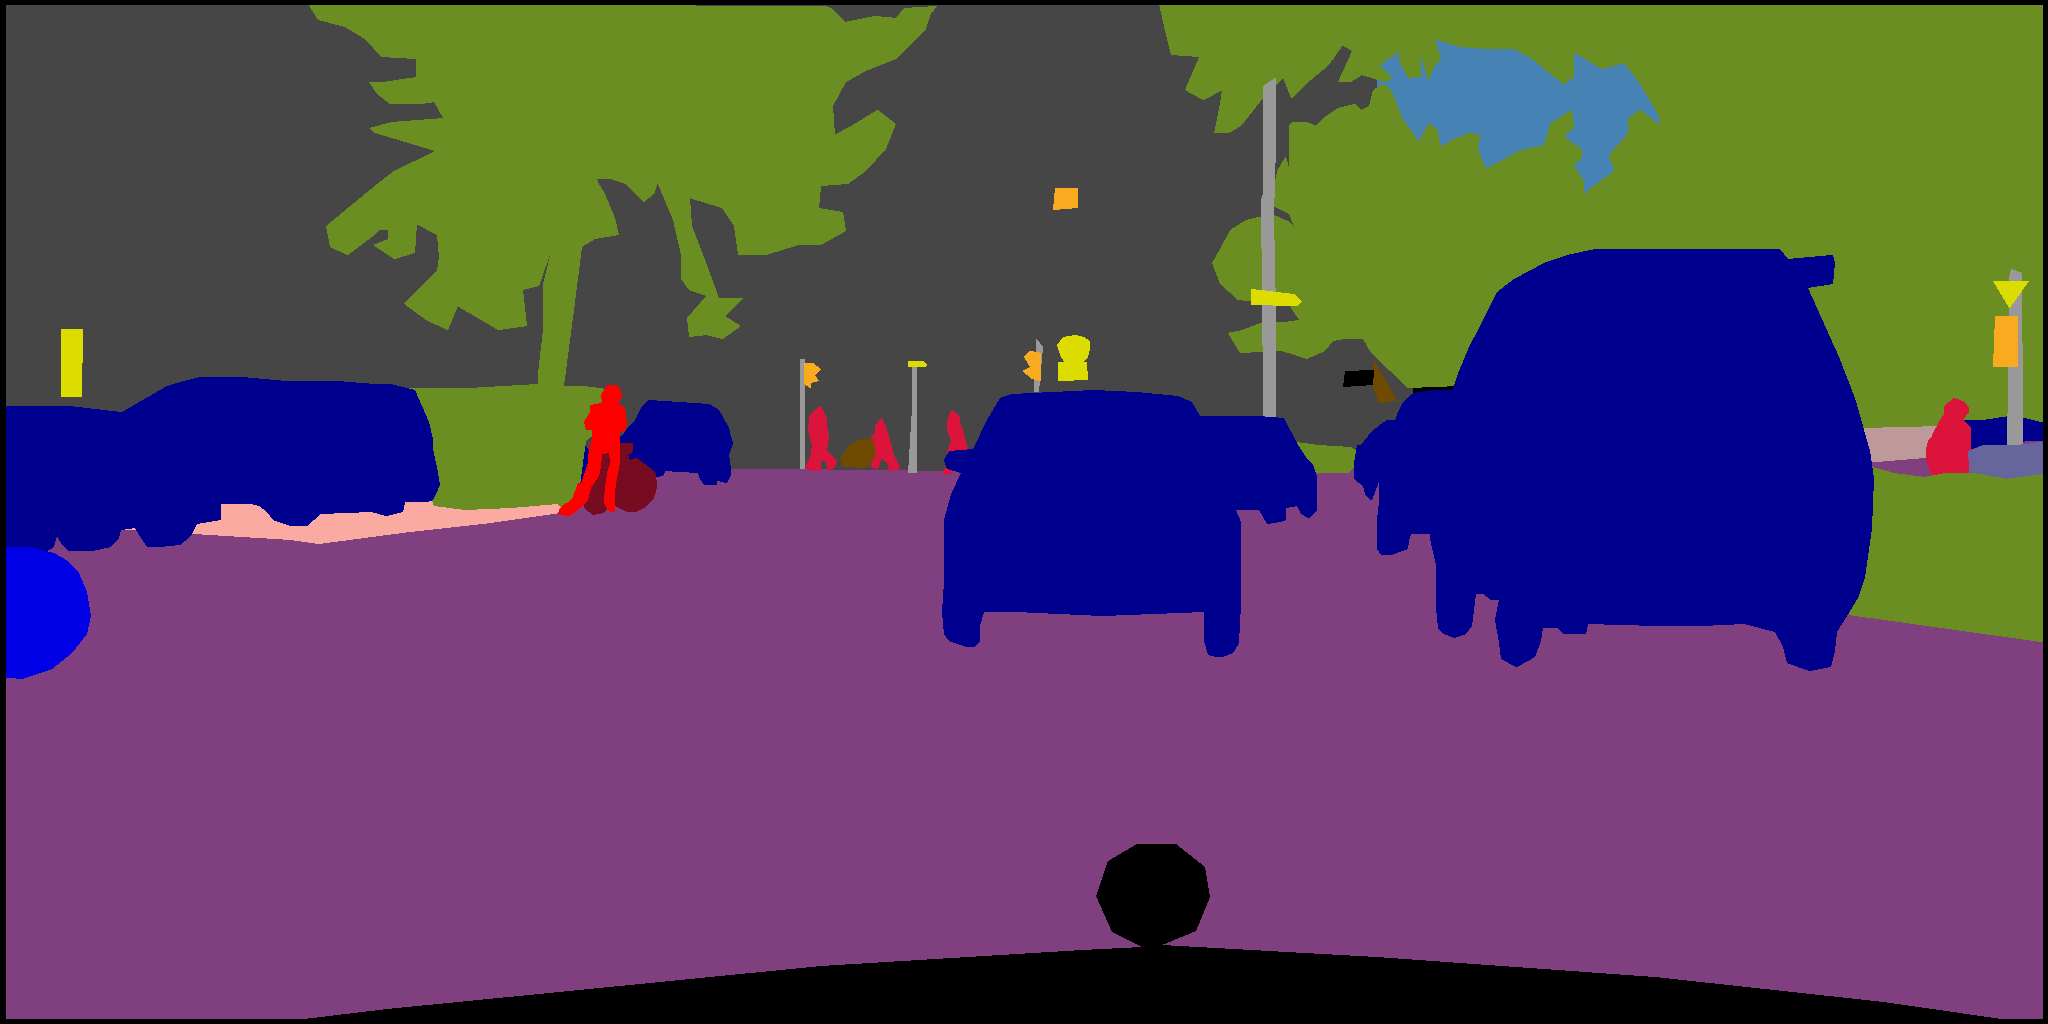
\includegraphics[width=0.40\textwidth]{zurich_example_seg.png}
\caption{Here is an illustration of fine annotated urban scene from Cityscapes Dataset. The upper side is an original image with 2048$\times$1024 resolution taken from Zuerich. The bottom side is its corresponding fine annotation. The overlayed color represents semantic classes defined by the dataset provider.}
\label{fig:leadfigure}
\end{figure}

\section{Related Work}
Proven classification architectures such as AlexNet and VGG (and their successors) are widely used for single-object recognitions. However, segmentation requires pixel-wise output to distinguish different objects rather than a single judgement. In 2015, Long et al. \cite{Long_2015_CVPR} introduced fully convolutional networks to adapt those classifiers for dense prediction, with in-network up-sampling and a pixel-wise loss. Therefore, by converting and fine tuning currently existing convolutional neural networks, it is possible to achieve a much better performance of segmentation than other simple methods such as k-means clustering and watershed transform.

Since this project is going to play a role among the problems of autonomous driving, Cityscapes Dataset \cite{Cordts2016Cityscapes} will be used in this project. It has fine annotated images and more coarse annotated images of urban scenarios from multiple cities. We will firstly use the 5000-image volumn including 3475 pixel-level fine annotated images for training and validation, and 1525 dummy annotated images for testing. The dummy annotation means regions are ignored. Class labels are defined and also grouped semantically. This dataset can be very useful due to its high quality and images resources (multiple cities). The dataset also have benchmarks for pixel-level and instance-level semantic labeling. They can be used to show segmentation performance quantitatively.


%-------------------------------------------------------------------------
\section{Model Structure}
VGG-16 has an outstanding performance on many datasets such as ImageNet for purposes of object recognition. Although casting VGG-16 \cite{Simonyan14c} to a fully convolutional network in the way described by \cite{Long_2015_CVPR} does handle the task for image segmentation, the resolution of segmentation is not good enough even if the training input has high resolutions. Therefore, we cast VGG-16 to an FCN with combinations of upsampling (unpooling) and convolutional layers (decoders) appended after convolutional layers by following the method described in \cite{badrinarayanan2015segnet2}.

\subsection{Network Structure}
First of all, we follow the structure of VGG-16 with batch normalization but simply discard the fully connected layers of it. Then, we append a set of unpooling and convolutional layers symmetrically to the convolutional layers, but with the output channel equal to the number of classes for the last layer. At the end of the network, we add a softmax function to produce class predictions for each pixel in the input image. That is, for each pixel, the network will give a probability distribution telling the likelihood of belonging to each class. This is an analog to the case of image classification, but is actually performing pixel-wise classifications.

In addition, we also add $``$links$"$ between each corresponding pooling and unpooling layers. This means the unpooling layers are deterministic with respect to max-pooling layers. When data goes through pooling layers, we record the indices of preserved pixels (or tensor elements). When doing unpooling, we place tensor elements back to the same places according to the previously recorded indices.

Therefore, the image input to the network is a tensor of size B$\times$C$\times$H$\times$W while the label (mask) input to it is a tensor of size B$\times$H$\times$W, where B, C, W, H stand for batch size, number of channels, image width, and image height respectively. The output of the network is a tensor of size B$\times$N$\times$H$\times$W where N stands for number of classes.

\subsection{Loss Function}
The loss function for this segmentation purpose is 2D cross-entropy loss. The idea is the same as the case of image classifications. Let P be the output (predictions) of the network, and have size N$\times$H$\times$W, and M of size H$\times$W be the ground-truth label of the segmented image; then the loss is defined as the following:
\begin{center}
	Loss = $-\sum_{i=0}^{W}\sum_{j=0}^{H}logP(M(j,i),j,i)$.
\end{center}
With this loss function, we use Adam to train the network model.

\begin{figure}[t]
	\centering
	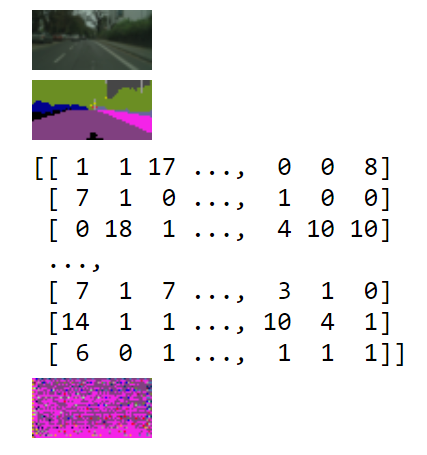
\includegraphics[width=0.50\textwidth]{bad_result.PNG}
	\caption{Here is a bad sample segmentation result of the trained neural network. The top is the original image. The second is the ground-truth label. The third (matrix) is the class predictions for each pixel on the original image. The bottom is the visualized class predictions.}
	\label{fig:leadfigure}
\end{figure}

\section{Experiments}
When training the network defined above, we use 3225 fine-annotated images as the training set and the rest 250 fine-annotated images as the validation set. There are also a test set available but the ground-truth labels are only available on the server of Cityscapes website. We have written a dataloader for CityScapes that can handle the whole fine-annotated dataset, including image transformations.

\subsection{Dataset Modifications}
As mentioned in \cite{Cordts2016Cityscapes}, only 19 classes frequently appear in those images, therefore the benchmark will only consider those 19 classes to avoid ambiguity. In this project, we discard labels other than the 19 classes by setting those discarded labels to the same value 255. When doing segmentation, those classes will be considered as the same "unknown" class.

Since the images in the dataset have a high resolution (2048$\times$1024), we resize them to 256$\times$128 in order to save time and graphic memories. When resizing the images, we use the default bicubic method. When resizing the masks (labels), we use nearest neighbors.


{\small
\bibliographystyle{ieee}
\bibliography{egbib}
}

\end{document}
